\documentclass[11pt,a4paper]{article}
\usepackage[utf8]{inputenc}
\usepackage{titlesec}
\usepackage[hidelinks]{hyperref}
\usepackage{pdfpages}
\usepackage{listings}
\usepackage{graphicx}
\usepackage{fullpage}

\newcommand{\sectionbreak}{\clearpage}
\renewcommand\contentsname{Inhaltsverzeichnis}
\renewcommand{\figurename}{Screenshot}

\begin{document}
\lstset{language=C}
\pagenumbering{roman}

\includepdf{titlepage.pdf}

\clearpage
\setcounter{page}{1}
\tableofcontents

\section{Aufgabe 1}
\pagenumbering{arabic}
\setcounter{page}{1}
Testprogramm \texttt{a1.c} bzw. \texttt{a1.cpp}:
\begin{lstlisting}[frame=single]
int add_five(int x);

int main() {
        int x = 3, res;
        res = add_five(x);
        return 0;
        }

int add_five(int x) {
        int add = 5;
        char c[10] = "AAAAAAAAA";
        return x + add;
        }
\end{lstlisting}
\subsection{Vorgehensweise}
\textbf{Compiler:} Obiges Programm mit gcc und g++ compiliert, jeweils mit Parameter \texttt{-fstack-protector}, \texttt{-fno-stack-protector} oder keinem von beiden.\\
\\
\textbf{Debugger:} In gdb einen Breakpoint ans Ende der Methode \texttt{add\_five} gesetzt, das Programm ausgeführt und den Stack betrachtet, zudem den disassemblierten Code inspiziert. Siehe Screenshot \ref{gcc0} auf Seite \pageref{gcc0}, Screenshot \ref{gcc1} auf Seite \pageref{gcc1}, Screenshot \ref{gpp0} auf Seite \pageref{gpp0} und Screenshot \ref{gpp1} auf Seite \pageref{gpp1}.
\subsection{Beobachtungen}
Sowohl bei gcc als auch g++ (auf dem vorliegenden System beide Version 4.4.5-8) entspricht das Verhalten von \texttt{-fno-stack-protector} dem Default. Die Position lokaler Variablen von Prozeduren sind bei beiden Compilern gleich, einige Werte auf dem Stack unterscheiden sich dagegen. Der Unterschied zwischen \texttt{-fstack-protector} und \texttt{-fno-stack-protector} ist in beiden Fällen deutlich erkennbar. Es werden beim Compilieren zusätzliche Maschinenbefehle generiert und der Aufbau des Stack ist verschieden.

\begin{figure}[h!]
  \caption{gcc mit Parameter \texttt{stack-protector}}
  \label{gcc0}
  \centering
    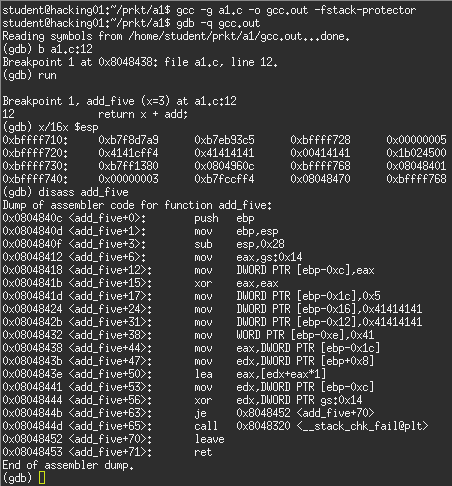
\includegraphics[scale=0.5]{1_gcc_protector_0.png}
\end{figure}
\begin{figure}[h!]
  \caption{gcc mit Parameter \texttt{no-stack-protector}}
  \label{gcc1}
  \centering
    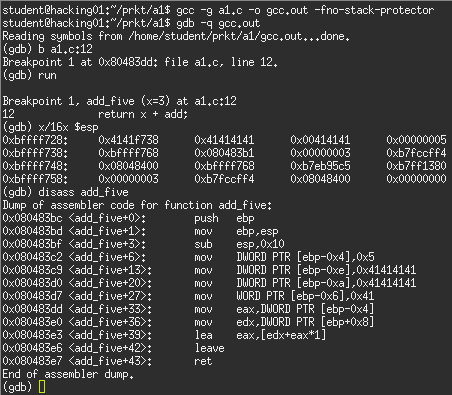
\includegraphics[scale=0.5]{1_gcc_protector_1.png}
\end{figure}
\begin{figure}[h!]
  \caption{g++ mit Parameter \texttt{stack-protector}}
  \label{gpp0}
  \centering
    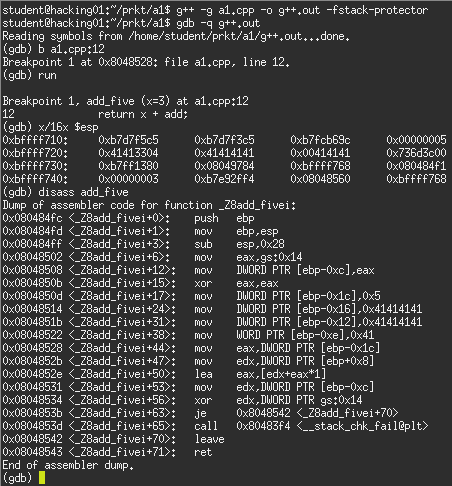
\includegraphics[scale=0.5]{2_gpp_protector_0.png}
\end{figure}
\begin{figure}[h!]
  \caption{g++ mit Parameter \texttt{no-stack-protector}}
  \label{gpp1}
  \centering
    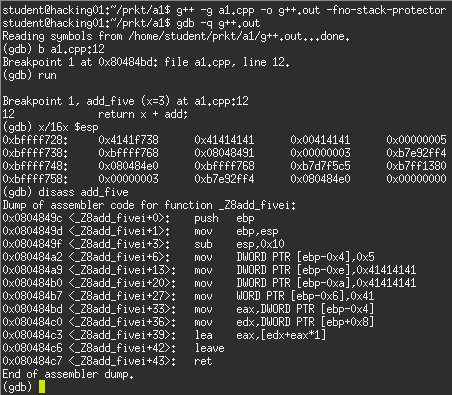
\includegraphics[scale=0.5]{2_gpp_protector_1.png}
\end{figure}


\section{Aufgabe 2}
\subsection{src\_audit\_1.c}
\subsubsection{Funktionsweise des Codeausschnitts}
Die Funktion \texttt{ownme1} nimmt zwei char-Pointer (\texttt{*in} und \texttt{*out}) für Strings und ein size\_t \texttt{maxout} entgegen. Die Funktion bricht ab, wenn \texttt{strlen(in)} größer ist als \texttt{maxout} oder \texttt{*in} nicht mit \# beginnt. Für jeden weiteren Wert in \texttt{*in} ungleich 0 wird:
\begin{itemize}
\item \$: kein weiteres Zeichen in \texttt{*out} geschrieben
\item \^{}: 15 mal "S\_" in \texttt{*out} geschrieben
\item sonst: ein Zeichen von \texttt{*in} in \texttt{*out} geschrieben
\end{itemize}
Am Ende wird die Zahl der geschriebenen Zeichen zurückgegeben.
\subsubsection{Schwachstelle}
\texttt{maxout} wird nur gegen \texttt{strlen(in)} geprüft. Für jedes \^{} in \texttt{*in} wird \texttt{*out} aber mehrmals inkrementiert. Im vorherigen Aufruf von \texttt{strlen} zählt jedes \^{} in \texttt{*in} dagegen nur 1. Dadurch lässt sich über die Grenzen von \texttt{*out} hinaus schreiben. 
\subsection{src\_audit\_2.c}
\subsubsection{Funktionsweise des Codeausschnitts}
Die Funktion \texttt{ownme2} nimmt einen char-Pointer \texttt{*input} entgegen. Die ersten 4 Zeichen werden als size\_t \texttt{size} interpretiert und für den char-Pointer \texttt{ptr} size+1 Byte allokiert. Am Ende werden \texttt{strlen(input)} Zeichen aus \texttt{input} nach \texttt{ptr} kopiert und letztgenannter zurückgegeben.
\subsubsection{Schwachstelle}
Größe von \texttt{ptr} liegt komplett in der Hand der aufrufenden Routine. Außerdem wird beim zweiten memcpy die komplette Größe von \texttt{input} verwendet und die ersten vier Zeichen nicht abgezogen.
\subsection{src\_audit\_3.c}
\subsubsection{Funktionsweise des Codeausschnitts}
Die Funktion \texttt{ownme3} nimmt ein Feld von \texttt{infoz} Stukturen und ein size\_t \texttt{count}. In einer Schleife werden \texttt{count} \texttt{infoz} vom \texttt{infoz}-Feld \texttt{in} in \texttt{out} kopiert. Am Ende wird der \texttt{infoz}-Zeiger \texttt{storage}, welcher auf \texttt{out} zeigt, "weggespeicher" und die Anzahl der kopierten \texttt{infoz} zurückgegeben.
\subsubsection{Schwachstelle}
Beim Kopieren der \texttt{infoz} wird die Validität der Stukturen nicht überprüft, sondern einfach mit memcpy \texttt{sizeof(struct infoz)} große Blöcke kopiert. Daher können die Struktur-Member \texttt{setting} und \texttt{userid} von \texttt{name} aus überschrieben werden.\\
Außerdem kann \texttt{count} größer gewählt werden als die Länge von \texttt{input}, sodass weitere Speicherbereiche mit irgendwelchen anderen Inhalten in \texttt{out} geschrieben werden.
\section{Aufgabe 3}
Hauptprogramm zu src\_audit\_1.c, welches für die Parameter \texttt{*in} und \texttt{maxout} der Funktion \texttt{ownme1} Werte aus der Kommandozeile entgegennimmt.
\begin{lstlisting}[frame=single]
#include<stdio.h>
#include<string.h>

int main(int argc, char** argv) {
        /* args: self input maxout */
        if(argc < 3) {
                printf("too few arguments\n");
                return -1;
                }
        int i, check;
        for(i=0; i<argc; i++) {
                printf("argv[%d]: %s\n", i, argv[i]);
                }
        size_t max = atoi(argv[2]);
        if(max > 128) {
                printf("maxout value too high\n");
                return -1;
                }
        char out[128] = "";
        check = ownme1(argv[1], out, max);
        if(check > -1)
                printf("output: %s\n", out);
        else
                printf("error: %d\n", check);
        return 0;
        }

    <Inhalt von src_audit_1.c>

\end{lstlisting}
\subsection{Vorgehensweise}
Normales/gewolltes Verhalten der Funktion \texttt{ownme1} testen, daraufhin versuchen, unerwünschtes Verhalten (Absturz) hervorzurufen (siehe Screenshot \ref{a3_0} auf Seite \pageref{a3_0}).
\begin{figure}[h!]
  \caption{Test des Hauptprogramms zu \texttt{ownme1}}
  \label{a3_0}
  \centering
    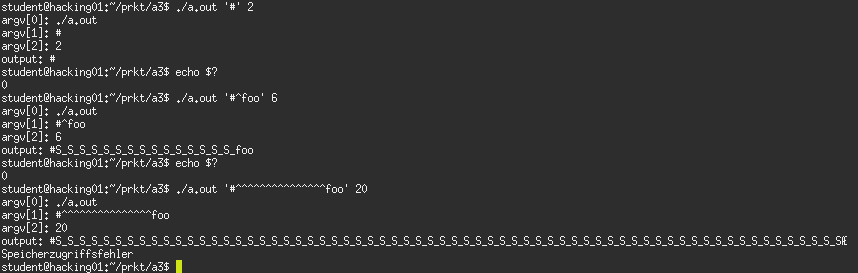
\includegraphics[scale=0.5]{a3_0.png}
\end{figure}
\section{Aufgabe 4}
\subsection{Vorgehensweise}
\begin{itemize}
\item \textbf{Code versehen}\\
Passwortabfrage innerhalb einer Funktion mit char-Feld, das einen Überlauf ermöglicht. Ziel: Rücksprungadresse der Funktion mit der einer anderen überschreiben.
\item \textbf{Compilieren}\\
\texttt{gcc -g overflow.c}
\item Zum Test einen Überlauf erzeugen, der zu einem Absturz führt (siehe Screenshot \ref{a4_0} auf Seite \pageref{a4_0}).
\item \textbf{Erwünschte Rücksprungadresse ermitteln}\\
\texttt{gdb -q a.out}\\
\texttt{disas go\_shell} $\rightarrow$ \texttt{0x080484d4}\\
(Siehe auch Screenshot \ref{a4_1} auf Seite \pageref{a4_1}
\item Betrachten des Stack-Layouts um zu ermitteln, wie weit das char-Feld überschrieben werden muss (siehe Screenshot \ref{a4_2} auf Seite \pageref{a4_2})
\item Exploit zur Kontrolle innerhalb von gdb durchführen (siehe Screenshot \ref{a4_3} auf Seite \pageref{a4_3})\\
Oder alternativ direkt: \texttt{perl -e 'print "A"x76; print "\textbackslash xd4\textbackslash x84\textbackslash x04\textbackslash x08"' | ./a.out}.
\end{itemize}
\begin{figure}[h!]
  \caption{Absturz durch manuelle Eingabe}
  \label{a4_0}
  \centering
    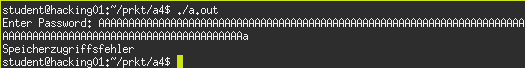
\includegraphics[scale=0.5]{a4_0.png}
\end{figure}
\begin{figure}[h!]
  \caption{Ermitteln der erwünschten Rücksprungadresse}
  \label{a4_1}
  \centering
    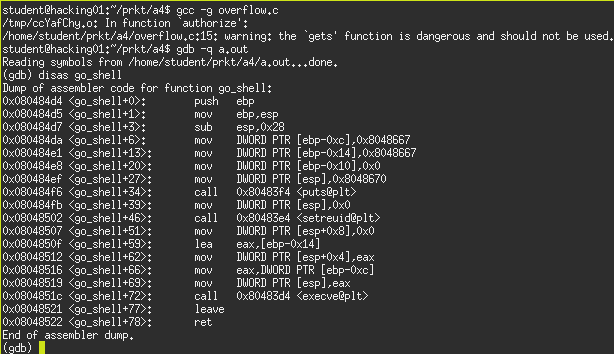
\includegraphics[scale=0.5]{a4_1.png}
\end{figure}
\begin{figure}[h!]
  \caption{Betrachten des Stack-Layouts}
  \label{a4_2}
  \centering
    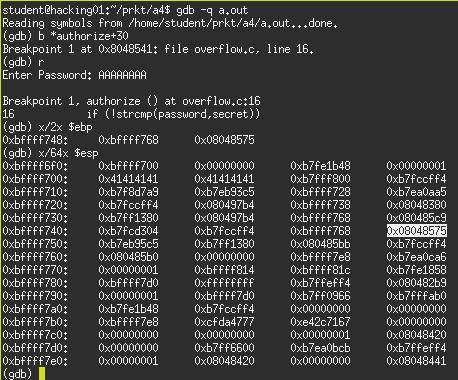
\includegraphics[scale=0.5]{a4_2.png}
\end{figure}
\begin{figure}[h!]
  \caption{Exploit}
  \label{a4_3}
  \centering
    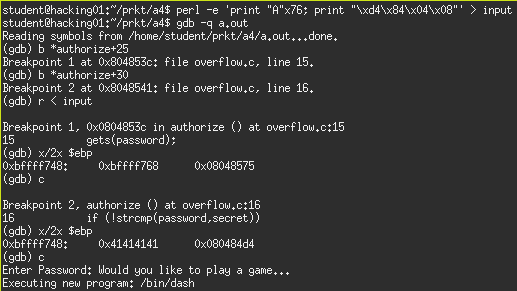
\includegraphics[scale=0.5]{a4_3.png}
\end{figure}
\section{Aufgabe 5}
\section{Aufgabe 6}

\end{document}
